\documentclass{beamer}
\usetheme{Boadilla}
\title{Ruby}
\author{Jarne Peters}
\date{\today}
\usepackage{graphicx}
\usepackage{tikz}


\begin{document}

\begin{frame}
\titlepage
\end{frame}

\section{Ruby}



\begin{frame}{Ruby}
\begin{tikzpicture}[overlay, remember picture]
  \node[anchor=north east, inner sep=0pt] at (current page.north east) {
\includegraphics[width=0.22\textwidth]{header-ruby-logo.png}};
\end{tikzpicture}
  \begin{itemize}

    \item 1995 von Yukihiro Matsumoto entwickelt.
    \item Motivation: Kombination der besten Features aus Perl, Smalltalk, Lisp und Python.
    \item Einzigartig durch Dynamik und Interpretierbarkeit.
    \item Elegante Organisation von Daten und Funktionen in Form von Objekten.
    \item Ruby ist vor allem wegen seiner einfachen Nutzung beliebt.
    \item Yukihiro Matsumoto legte besonders großen Wert darauf, dass Programmieren mit Ruby Spaß macht.
  \end{itemize}
\end{frame}

\begin{frame}{Ruby Syntax}
  \begin{itemize}
    \item Die Syntax von Ruby ähnelt der von Perl oder Python.
    \item Klassen und Methoden werden durch Schlüsselwörter gekennzeichnet.
    \item Variablen in Ruby benötigen keinen Sigil als Präfix (im Gegensatz zu Perl).
    \item Instanzvariablen sind vollständig privat für die Klassen und können nur durch bestimmte Methoden offengelegt werden.
    \item Ruby zeichnet sich durch Einfachheit und Ausdrucksstärke aus.
    \item Semikolons am Zeilenende sind nicht notwendig.
    \item Variablen werden durch ein vorangestelltes Dollarzeichen oder Kleinbuchstaben dargestellt.
    \item Typen werden dynamisch interpretiert.
  \end{itemize}
\end{frame}
\begin{frame}{Blöcke in Ruby}
  \begin{itemize}
    \item Blöcke in Ruby ermöglichen die Erstellung anonymer Funktionen und deren Weitergabe an Methoden.
    \item Sie können durch das `do..end`-Statement oder geschweifte Klammern `\{\}` definiert werden.

    \item Die Verwendung von Blöcken führt zu kompaktem und wiederverwendbarem Code.
    \item Das Schlüsselwort `yield` ruft den Code innerhalb des Blocks auf

  \end{itemize}
\begin{tikzpicture}[overlay, remember picture]
  \node[anchor=south, inner sep=0pt] at (current page.south) {\includegraphics[width=0.6\textwidth]{block.png}};
\end{tikzpicture}

\end{frame}
\begin{frame}{Ruby Mixins}
\section*{Ruby Mixins:}

\begin{itemize}
  \item In Ruby keine Mehrfachvererbung, stattdessen Module als Mixins.
  \item Mixins werden in Klassen eingefügt, um Funktionalitäten zu teilen, ohne direkte Vererbung.
  \item Im Gegensatz zur klassischen Vererbung erlaubt Ruby, mehrere Module in eine Klasse einzufügen.
  \item Module sind Sammlungen von Methoden, Konstanten und Ausdrücken.
  \item Mixins fördern Code-Wiederverwendbarkeit und erleichtern die Strukturierung.
  \item Reduzieren Redundanz, ermöglichen flexible Hinzufügung von Funktionen ohne komplexe Vererbungshierarchien.
  \item Leistungsstarkes Feature für Wiederverwendbarkeit und Flexibilität ohne Beeinträchtigung der klaren Struktur.
\end{itemize}
\end{frame}
\begin{frame}{Ruby Mixins}
\section*{Ruby Mixins:}

\begin{tikzpicture}[overlay, remember picture]
  \node[anchor=south, inner sep=0pt] at (current page.south) {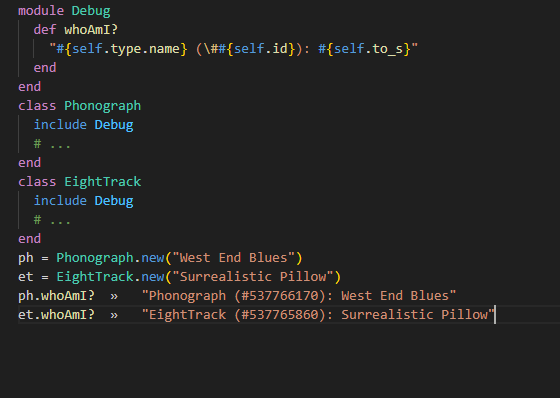
\includegraphics[width=1\textwidth]{mixins.png}};
\end{tikzpicture}

\end{frame}

\begin{frame}{Entwicklung von Ruby}
  \begin{itemize}
    \item Als Open-Source-Programmiersprache ermöglicht Ruby Entwicklern weltweit, am Code mitzuwirken und Verbesserungen vorzuschlagen.
    \item Der Quellcode von Ruby wird auf GitHub gehostet.
    \item Interessierte können sich der Mailingliste von Ruby anschließen, um aktiv an der Entwicklung teilzunehmen.
    \item Die Mailingliste teilt wichtige Informationen, Diskussionen und Entscheidungen zur Weiterentwicklung der Sprache.
    \item Die Veröffentlichung von Ruby-Updates erfolgt in der Regel jährlich um die Weihnachtszeit.
  \end{itemize}
\end{frame}
\begin{frame}{Dokumentation von Ruby}
  \begin{itemize}
    \item Die Ruby-Dokumentation ist die beste Ressource für Entwickler, um die Sprache effektiv zu lernen, zu verstehen und zu nutzen.
    \item Die offizielle Website von Ruby bietet eine umfassende Dokumentation sowohl für Anfänger als auch für erfahrene Entwickler.
    \item Neben grundlegenden Informationen bietet die Website detaillierte Anleitungen, Tutorials und Referenzmaterialien.
  \end{itemize}
\end{frame}

\begin{frame}{IDEs for Ruby}
  \begin{itemize}
    \item Es gibt eine Reihe integrierter Entwicklungsumgebungen (IDEs), die die Ruby-Programmierung unterstützen.
    \item Bekannte IDEs für Ruby sind:
      \begin{itemize}
        \item Visual Studio Code
        \item Sublime Text
        \item AWS Cloud9
        \item RubyMine (von JetBrains speziell für Ruby entwickelt)
      \end{itemize}
    \item RubyMine ist kostenpflichtig, während einige der anderen genannten IDEs kostenlos verfügbar sind.
  \end{itemize}
\end{frame}
\begin{frame}{RubyGems: Package Management in Ruby}
  \begin{itemize}
    \item RubyGems stellt ein standardisiertes Format für die Bereitstellung von Bibliotheken und Programmen namens Gems bereit.
    \item RubyGems wird als standardisiertes Format bereitgestellt, das Entwicklern eine konsistente Möglichkeit bietet, ihre Gems oder Programme bereitzustellen und zu hosten.
    \item Dies stellt sicher, dass Gems konsistent formatiert sind und ermöglicht einen reibungslosen Austausch zwischen verschiedenen Projekten und Entwicklern.
    \item Gems werden mit dem Gem-Befehlszeilentool installiert, das der Ruby-Community eine benutzerfreundliche Schnittstelle bietet.
    \item Entwickler können die erforderlichen Bibliotheken herunterladen, installieren und in ihre Projekte integrieren, indem sie einfach ein paar Befehle ausführen.
    \item RubyGems ist seit Ruby Version 1.9 in der Standard-Ruby-Distribution enthalten.
  \end{itemize}
\end{frame}
\begin{frame}{Andere Ruby-Implementierungen}
  \begin{itemize}
    \item Ruby hat nicht nur eine Implementierung, sondern viele.
    \item Die Standardimplementierung wird als MRI (Matz's Ruby Interpreter) oder Cruby bezeichnet, da sie in C geschrieben ist.
    \item Es gibt alternative Implementierungen mit verschiedenen Features und Funktionen.
    \item JRuby basiert auf der Java Virtual Machine (JVM) und ermöglicht die Nutzung von JVM-spezifischen Funktionen.
    \item Rubinius ist in Ruby selbst geschrieben und baut auf LLVM auf, was neue Möglichkeiten für die Ruby-Entwicklung eröffnet.
    \item Truffle Ruby ist eine leistungsstarke Implementierung, die mit dem Truffle-Framework entwickelt wurde, um die Laufzeitleistung und Ressourcennutzung zu verbessern.
    \item Jede Implementierung bietet einzigartige Vorteile und Funktionen, die die Vielfalt der Ruby-Entwicklung bereichern.
    \item Die Wahl der Implementierung hängt oft von den spezifischen Anforderungen des Projekts ab, sei es in Bezug auf Leistung, Plattformintegration oder andere Faktoren.
  \end{itemize}
\end{frame}
\begin{frame}{Ruby Interpreter}
  \begin{itemize}
    \item Ruby ist eine interpretierte Programmiersprache.
    \item Erste Generation von Ruby-Interpretern war MRI (Matz's Ruby Interpreter) bis Version 1.9.
    \item MRI wurde von Yukihiro Matsumoto in C geschrieben, war aber aufgrund des Global Interpreter Lock (GIL) nur begrenzt für parallele Programmierung geeignet.
    \item In Version 1.9 wurde MRI durch YARV (Yet Another Ruby VM) ersetzt, der einen JIT-Compiler einführte und die Codeausführung beschleunigte.
    \item GIL bleibt erhalten, wodurch echte parallele Ausführung von Ruby-Threads nicht möglich ist.
    \item Alternative Ruby-Implementierungen stehen zur Verfügung, um verschiedene Funktionen, Leistungsoptimierungen und parallele Unterstützung zu bieten.
  \end{itemize}
\end{frame}
\begin{frame}{Ruby Community}
  \begin{itemize}
    \item Ein bedeutender Bestandteil der Ruby-Welt ist die Ruby-Community.
    \item Die Community unterstützt die Weiterentwicklung der Sprache und bietet Hilfe durch zahlreiche von der Community entwickelte Gems.
    \item Auf der Ruby-Homepage gibt es eine Vielzahl von Links zu Ruby User Groups, in denen sich Programmierende austauschen und organisieren können.
    \item Die Mailingliste von Ruby ist ein wichtiger Austauschpunkt für aktive Mitarbeit an der Ruby-Entwicklung. Es gibt englischsprachige und sogar eine deutschsprachige Mailingliste.
    \item Jährliche Ruby-Konferenzen bieten Plattformen für den Wissensaustausch und die Vernetzung innerhalb der Ruby-Community.
    \item Beispiele sind die EuRuKo (European Ruby Conference), die RubyConf in den USA und die RubyKaigi in Japan.
  \end{itemize}
\end{frame}
\begin{frame}{Ruby on Rails}

Entwicklung und Einführung:
  \begin{itemize}
    \item Ruby on Rails (Rails) ist ein Web Application Framework, entwickelt in der Programmiersprache Ruby.
    \item Veröffentlicht 2004, schnell an Beliebtheit gewonnen durch innovative Features.
  \end{itemize}


Model-View-Controller (MVC)-Muster:

  \begin{itemize}
    \item Grundlegendes Konzept, strukturiert Anwendungen in Modell, Controller und Ansicht.
    \item Modell repräsentiert Daten und Beziehungen, Controller handhabt Anfragen, Ansicht visualisiert Daten.
  \end{itemize}

  \begin{itemize}
    \item "Don't Repeat Yourself" (DRY): Informationen nur einmal in der Datenbank, fördert Code-Wiederverwendbarkeit.
    \item "Convention over Configuration": Sinnvolle Standardwerte, minimiert Konfiguration, spart Entwicklungszeit.
  \end{itemize}
\end{frame}



\begin{frame}{Ruby on Rails}
  \begin{itemize}
  \item Fokus auf der Freude am Programmieren, Spaß bei der Entwicklung von Anwendungen.
    \item APIs nach dem "Bigger Smile" Prinzip gestaltet, um Entwicklern ein positives Erlebnis zu bieten.
    \item Plattformen wie GitHub, Shopify und Twitch nutzen Ruby on Rails.
  \end{itemize}
\end{frame}
\begin{frame}{Grep Clone Implementation}
  \begin{itemize}
    \item Umsetzung eines Grep-Klons in drei Hauptabschnitten.
    \item Optionen, Matching und parallele Ausführung.
    \item Verwendung der OptionParser-Bibliothek für die Definition von Befehlszeilenoptionen.
    \item Farbliche Hervorhebung von Treffern durch Integration der Colorize-Bibliothek.
    \item Hauptfunktion \texttt\{search\_file\} verarbeitet Dateien in Chunks, minimiert Speicherverbrauch.
    \item Parallelisierung mit der Parallel-Bibliothek für effiziente Ausführung.
    \item Implementierung von before\_context- und after\_context-Optionen für Kontextausgabe.
   
  \end{itemize}
\end{frame}
\begin{frame}{Grep Clone Implementation}
  \begin{itemize}
    
    \item Suche nach regulären Ausdrücken mit der \texttt\{match\}-Methode
    \item Leistungsanalyse mit dem Benchmark-Gem und Identifizierung von Verbesserungsmöglichkeiten.
    \item Herausforderungen waren Leistungsproblemen und Einschränkungen des MRI-Interpreters.
    \item Programmiererlebnis mit Ruby ist angenehm und leicht verständlich.
    \item Klar strukturierte Syntax und hohe Lesbarkeit erleichtern den Entwicklungsprozess.
    \item Ruby bietet einen unkomplizierten Einstieg in die Programmierung, besonders für erfahrene Entwickler.
  \end{itemize}
\end{frame}
\begin{frame}{Grep Clone Implementation}
\vspace{-\topsep}
\begin{itemize}
\item Umsetzung der Optionen mittels Optionparse
\end{itemize}
  \begin{tikzpicture}[overlay, remember picture]
  \node[anchor=center, inner sep=0pt] at (current page.center) {\includegraphics[width=\paperwidth, height=\paperheight, keepaspectratio]{optionen.png}};
\end{tikzpicture}

  
\end{frame}
\begin{frame}{Grep Clone Implementation}
 \begin{itemize}
\item Einteilung in Chunks und erstellen von Regular Expressions
\end{itemize}
   \begin{tikzpicture}[overlay, remember picture]
  \node[anchor=center, inner sep=0pt] at (current page.center) {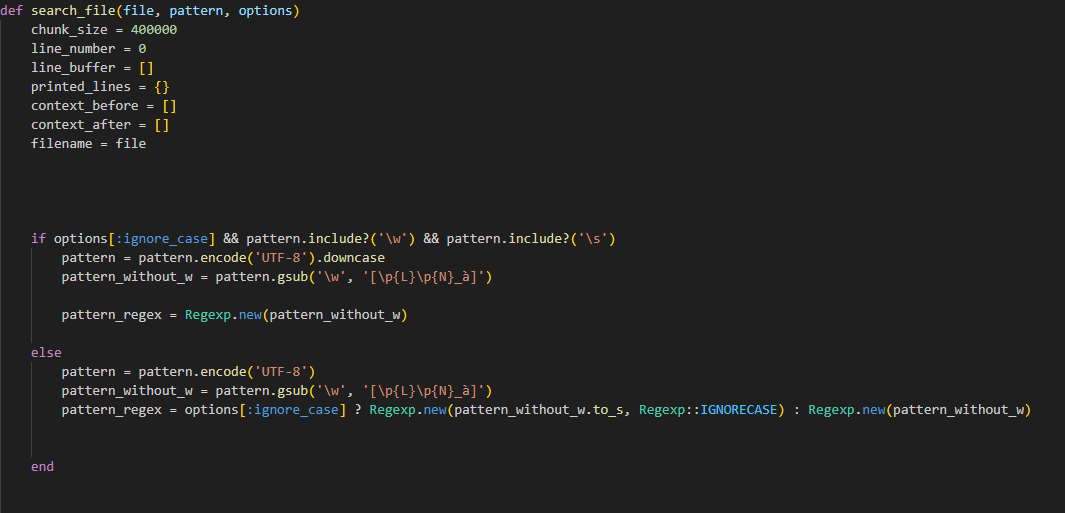
\includegraphics[width=\paperwidth, height=\paperheight, keepaspectratio]{chunks.png}};
\end{tikzpicture}
\end{frame}
\begin{frame}{Grep Clone Implementation}
 \begin{itemize}
\item Umsetzungvon before\_context
\end{itemize}
   \begin{tikzpicture}[overlay, remember picture]
  \node[anchor=center, inner sep=0pt] at (current page.center) {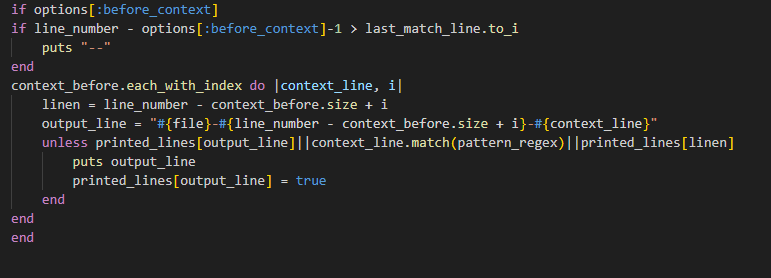
\includegraphics[width=\paperwidth, height=\paperheight, keepaspectratio]{before.png}};
\end{tikzpicture}
\end{frame}
\begin{frame}{Grep Clone Implementation}
 \begin{itemize}
\item Einteilung in Chunks und erstellen von Regular Expressions
\end{itemize}
   \begin{tikzpicture}[overlay, remember picture]
  \node[anchor=center, inner sep=0pt] at (current page.center) {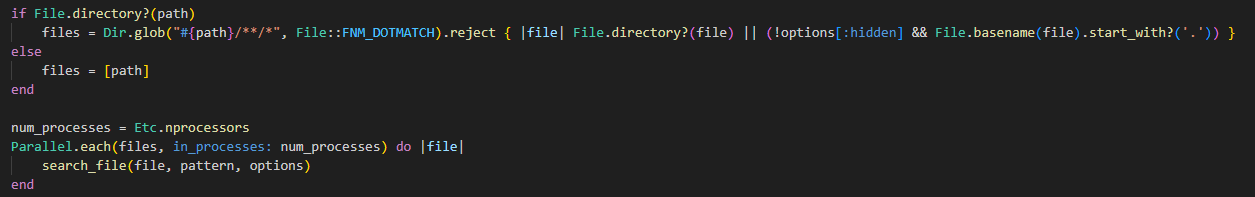
\includegraphics[width=\paperwidth, height=\paperheight, keepaspectratio]{parallel.png}};
\end{tikzpicture}
\end{frame}
\begin{frame}{Fazit: Die Vielseitigkeit und Zukunft von Ruby}
  \begin{itemize}
    \item Ruby hat sich als vielseitig und einflussreich in verschiedenen Anwendungsbereichen bewiesen.
    \item Klare Syntax, Flexibilität und Fähigkeit zur Erstellung eleganter, lesbare Codes.
    \item Besonderer Fokus auf Webentwicklung durch das beliebte Ruby on Rails-Framework.
    \item Einfachheit und Lesbarkeit von Ruby-Code erleichtern den Einstieg und effizientes Programmieren.
    \item Ruby wird voraussichtlich eine bedeutende Rolle in der Softwareentwicklung beibehalten.
    \item Herausforderungen durch zunehmende Verwendung von Ruby on Rails im Vergleich zu anderen Frameworks.
    \item Trotzdem bleibt Ruby ein essenzieller Bestandteil der Programmierlandschaft mit anhaltender Innovation.
  \end{itemize}
\end{frame}
\begin{frame}{Quellen}
  \begin{itemize}
    \item https://www.ruby-lang.org/
    \item https://rubyonrails.org/
    \item https://www.jetbrains.com/de-de/lp/devecosystem-2021/ruby/
    \item https://ruby-doc.com/docs/ProgrammingRuby/html/tut\_modules.html
    \item https://ruby-doc.com/docs/ProgrammingRuby/html/tut\_modules.html
  \item https://rubygems.org
  \end{itemize}
\end{frame}
\end{document}